\section{Actores}

A continuación se describen los actores que se involucran, de una manera u otra,
con el sistema.

\begin{description}

\item[Cliente] \hfill \\
Solicita una tarjeta y realiza compras con ella.

\item[Comercio] \hfill \\
Realiza ventas de bienes y/o servicios al cliente, quien paga por ellos
utilizando la tarjeta.

\item[Administrador] \hfill \\
Configura y adminstra el sistema informático desarrollado manteniendo datos de
referencia como ser los comercios y clientes registrados.

\item[Mensualmente] \hfill \\
Actor temporal mensual involucrado en los procesos de generación de resúmenes de
cuenta por clientes y resúmenes de saldo por comercio.

\item[Diariamente] \hfill \\
Actor termporal diario involucrado en los procesos de verificación y renovación
de tarjetas vencidas.

\end{description}

\section{Diagrama de casos de uso} \label{sec:diagrama_casos_uso}

En la figura~\ref{fig:modcasosuso:diagramacasos} se exponen los actores
involucrados en la operación del sistema y su interacción con el mismo a través
de los casos de uso identificados. En secciones subsiguientes se detallará cada
uno de estos últimos.

\begin{figure}[htb]
\begin{center}
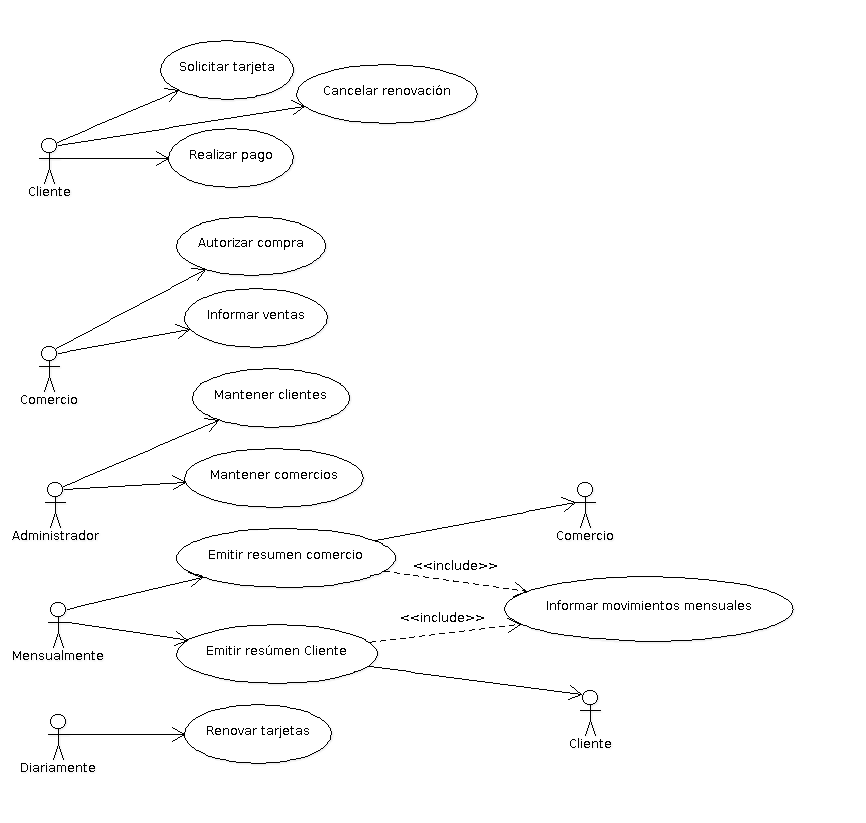
\includegraphics[width=0.9\textwidth]{images/mod_casosuso_diagrama.png}
\end{center}
\caption{Diagrama de casos de uso}
\label{fig:modcasosuso:diagramacasos}
\end{figure}

\FloatBarrier

\section{Detalle de casos de uso}

En esta sección se detallan cada uno de los casos de uso presentados en el
diagrama de casos de uso de la sección~\ref{sec:diagrama_casos_uso}.

\subsection{Solicitar tarjeta}
\begin{tabularx}{\textwidth}{| r | X |}
\hline
\multicolumn{2}{|X|}{
\textbf{Use Case}: Solicitar tarjeta} \\

\hline
\multicolumn{2}{|c|}{\cellcolor[gray]{0.6}} \\

\hline
\multicolumn{2}{|X|}{
\textbf{Descripción}: Registración de los datos de un cliente y emisión de una
tarjeta a su nombre.} \\

\hline
\multicolumn{2}{|X|}{
\textbf{Actores participantes}: Cliente} \\

\hline
\multicolumn{2}{|c|}{\cellcolor[gray]{0.6} } \\

\hline
\multicolumn{2}{|X|}{
\textbf{Flujos}} \\

\hline
\multicolumn{2}{|X|}{
\textbf{Flujo principal}} \\

\hline
1 & El cliente solicita una nueva tarjeta. \\
\hline
2 & El sistema solicita los datos del cliente. \\
\hline
3 & Se ingresan los datos del cliente (nombre, apellido, dni, límite de compra,
domicilio, teléfono). \\
\hline
4 & El sistema valida que el dni del cliente no haya sido registrado aún (E1.1
si ya ha sido registrado). \\
\hline
5 & El sistema pide confirmación de que el cliente ha presentado una fotocopia
de su dni (E2.1 si no se da confirmación). \\
\hline
6 & El sistema pide confirmación de que el cliente ha presentado la
documentación asociada a la garantía, y que esta es satisfactoria (E2.1 si no se
da confirmación). \\
\hline
7 & El sistema almacena los datos del cliente y genera un número de tarjeta. \\
\hline
8 & Fin del caso de uso. \\

\hline
\multicolumn{2}{|X|}{
\textbf{Flujos de excepción}} \\

\hline
E1.1 & El sistema emite un mensaje de error informando que el cliente ya posee
una tarjeta. \\
\hline
E1.2 & El caso de uso continua en 8 \\

\hline
E2.1 & El sistema emite un mensaje de error informando que el cliente no
presentó documentación obligatoria para continuar con la solicitud. \\
\hline
E1.2 & El caso de uso continua en 8 \\

\hline
\end{tabularx}



\subsection{Cancelar renovación}
\begin{tabularx}{\textwidth}{| r | X |}
\hline
\multicolumn{2}{|X|}{
\textbf{Use Case}: Cancelar renovación} \\

\hline
\multicolumn{2}{|c|}{\cellcolor[gray]{0.6}} \\

\hline
\multicolumn{2}{|X|}{
\textbf{Descripción}: Cancela el proceso de renovación automática de la tarjeta,
de manera que la tarjeta sigue vigente hasta que expire. A partir de su
expiración, la tarjeta se mantiene como inactiva y no puede ser utilizada.} \\

\hline
\multicolumn{2}{|X|}{
\textbf{Actores participantes}: Cliente} \\

\hline
\multicolumn{2}{|c|}{\cellcolor[gray]{0.6} } \\

\hline
\multicolumn{2}{|X|}{
\textbf{Flujos}} \\

\hline
\multicolumn{2}{|X|}{
\textbf{Flujo principal}} \\

\hline
1 & El cliente solicita la cancelación de la renovación automática de su
tarjeta. \\
\hline
2 & El sistema solicita el número de tarjeta del cliente. \\
\hline
3 & El sistema valida que el número de tarjeta del cliente exista (E1.1 si no
existe). \\
\hline
4 & El sistema valida que la tarjeta del cliente esté activa y su renovación no
haya sido cancelada (E2.1 si está inactiva o su renovación ya ha sido
cancelada). \\
\hline
5 & El sistema marca la tarjeta como "no renovar". Se mantiene activa, pero en
su fecha de expiración la tarjeta no se renovará automáticamente. \\
\hline
6 & Fin del caso de uso. \\

\hline
\multicolumn{2}{|X|}{
\textbf{Flujos de excepción}} \\

\hline
E1.1 & El sistema emite un mensaje de error informando que no existe una tarjeta
con el número de tarjeta ingresado \\
\hline
E1.2 & El caso de uso continua en 6 \\

\hline
E2.1 & El sistema emite un mensaje de error informando que la tarjeta está
inactiva o que su renovación ya ha sido cancelada. \\
\hline
E2.2 & El caso de uso continua en 6 \\

\hline
\end{tabularx}



\subsection{Realizar pago}
\begin{tabularx}{\textwidth}{| r | X |}
\hline
\multicolumn{2}{|X|}{
\textbf{Use Case}: Realizar pago} \\

\hline
\multicolumn{2}{|c|}{\cellcolor[gray]{0.6}} \\

\hline
\multicolumn{2}{|X|}{
\textbf{Descripción}: Registración de un pago a nombre de un cliente en
concepto de los consumos realizados durante el mes anterior.} \\

\hline
\multicolumn{2}{|X|}{
\textbf{Actores participantes}: Cliente} \\

\hline
\multicolumn{2}{|c|}{\cellcolor[gray]{0.6} } \\

\hline
\multicolumn{2}{|X|}{
\textbf{Flujos}} \\

\hline
\multicolumn{2}{|X|}{
\textbf{Flujo principal}} \\

\hline
1 & El cliente se presenta en las oficinas de pagos para pagar el monto
adeudado. \\
\hline
2 & El sistema solicita el DNI del cliente. (E1 si el cliente no existe). \\
\hline
3 & El sistema informa los datos del cliente para su validación, y solicita
confirmación de que estos son correctos (E2 si los datos no son correctos). \\
\hline
4 & El sistema informa el monto adeudado por el cliente. (S1 si el monto
adeudado es cero, S2 si la fecha del día no es del uno al diez de cada mes). \\
\hline
5 & El sistema solicita el importe abonado por el cliente y actualiza el saldo
de su cuenta corriente.\\
\hline
6 & Fin del caso de uso. \\

\hline
\multicolumn{2}{|X|}{
\textbf{Flujos alternativos}} \\

\hline
S1.1 & El sistema emite un mensaje informando que el cliente no posee saldo
adeudado. \\
\hline
S1.2 & El caso de uso continua en 6. \\

\hline
S2.1 & El sistema emite un mensaje informando que no se pueden registrar pagos
fuera de término, e indicando el próximo periodo en el que se podrán registrar
pagos (en las fechas uno al diez de cada mes). \\
\hline
S2.2 & El caso de uso continua en 6. \\


\hline
\multicolumn{2}{|X|}{
\textbf{Flujos de excepción}} \\

\hline
E1.1 & El sistema emite un mensaje de error informando que el cliente no
existe. \\
\hline
E1.2 & El caso de uso continua en 6. \\

\hline
E2.1 & El sistema emite un mensaje de error informando que no se registrará
ningún pago. \\
\hline
E2.2 & El caso de uso continua en 2. \\

\hline
\end{tabularx}



\subsection{Autorizar compra}
\begin{tabularx}{\textwidth}{| r | X |}
\hline
\multicolumn{2}{|X|}{
\textbf{Use Case}: Autorizar compra} \\

\hline
\multicolumn{2}{|c|}{\cellcolor[gray]{0.6}} \\

\hline
\multicolumn{2}{|X|}{
\textbf{Descripción}: Validación de las condiciones de uso de una tarjeta para
realizar un pago en un comercio adherido.} \\

\hline
\multicolumn{2}{|X|}{
\textbf{Actores participantes}: Comercio} \\

\hline
\multicolumn{2}{|c|}{\cellcolor[gray]{0.6} } \\

\hline
\multicolumn{2}{|X|}{
\textbf{Flujos}} \\

\hline
\multicolumn{2}{|X|}{
\textbf{Flujo principal}} \\

\hline
1 & El comercio requiere al sistema que este valide una tarjeta informando el
número de esta, el DNI del cliente y el importe de la venta que el cliente
quiere abonar utilizando la misma. \\
\hline
2 & El sistema realiza las siguientes validaciones (S1 si alguna de las
validaciones fallase). 
\begin{enumerate}
\item El número de tarjeta debe estar asociado a una tarjeta.
\item La tarjeta debe estar activa.
\item El DNI del cliente asociado a la tarjeta debe coincidir con el DNI
informado.
\item El saldo de la cuenta asociada a la tarjeta más el importe informado de
la venta no debe superar el límite de saldo asociado a la cuenta.
\end{enumerate} \\
\hline
3 & El sistema informa al comercio que la compra está autorizada. \\
\hline
4 & Fin del caso de uso. \\

\hline
\multicolumn{2}{|X|}{
\textbf{Flujos alternativos}} \\

\hline
S1.1 & El sistema informa al comercio que la compra no está autorizada,
adjuntando en el mensaje el motivo por el cual no se autoriza la misma. \\
\hline
S1.2 & El caso de uso continua en 4. \\

\hline
\end{tabularx}



